\section{Layout}

\begin{figure}[!htb]
	\minipage{0.45\textwidth}
		\centering
		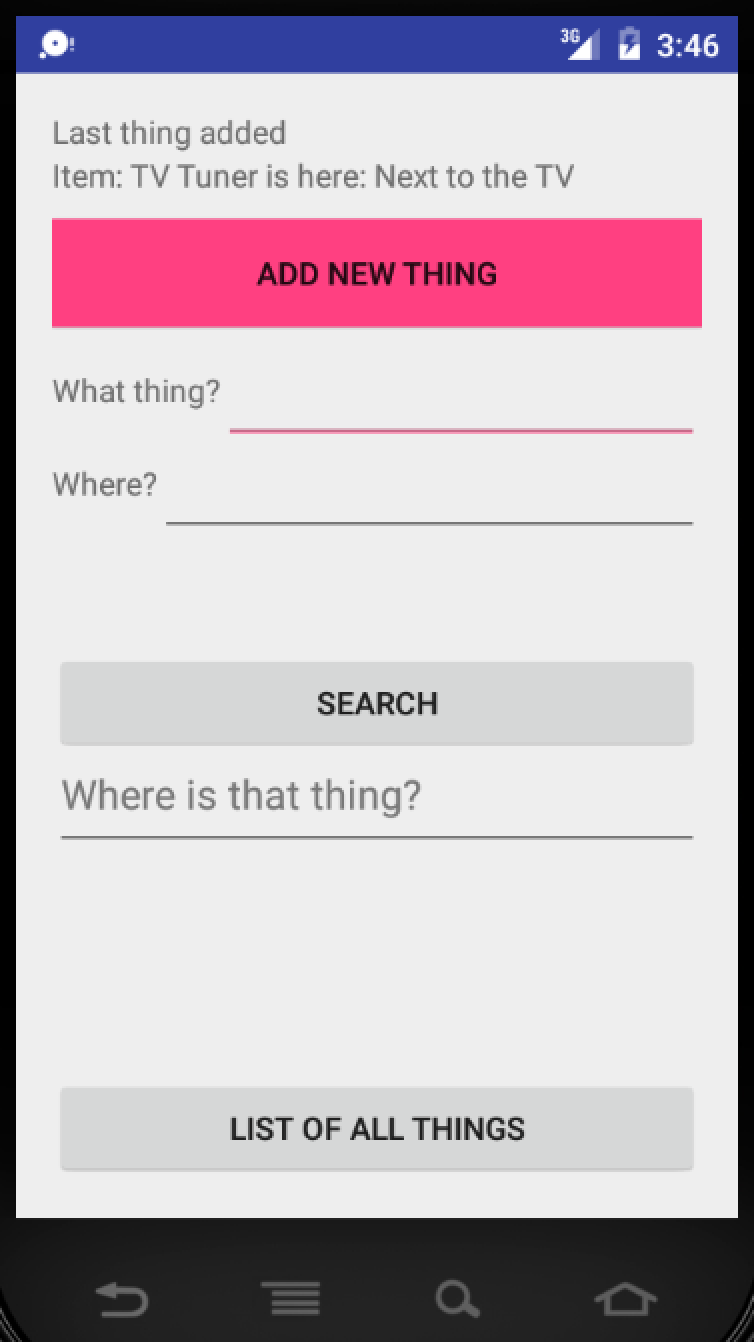
\includegraphics[width=0.9\linewidth]{Tingle-Portrait.png}
		\caption{The main view (Tingle Activity) in portrait mode.}
		\label{fig:tingle-view-portrait}
	\endminipage\hfill
	\minipage{0.45\textwidth}
		\centering
		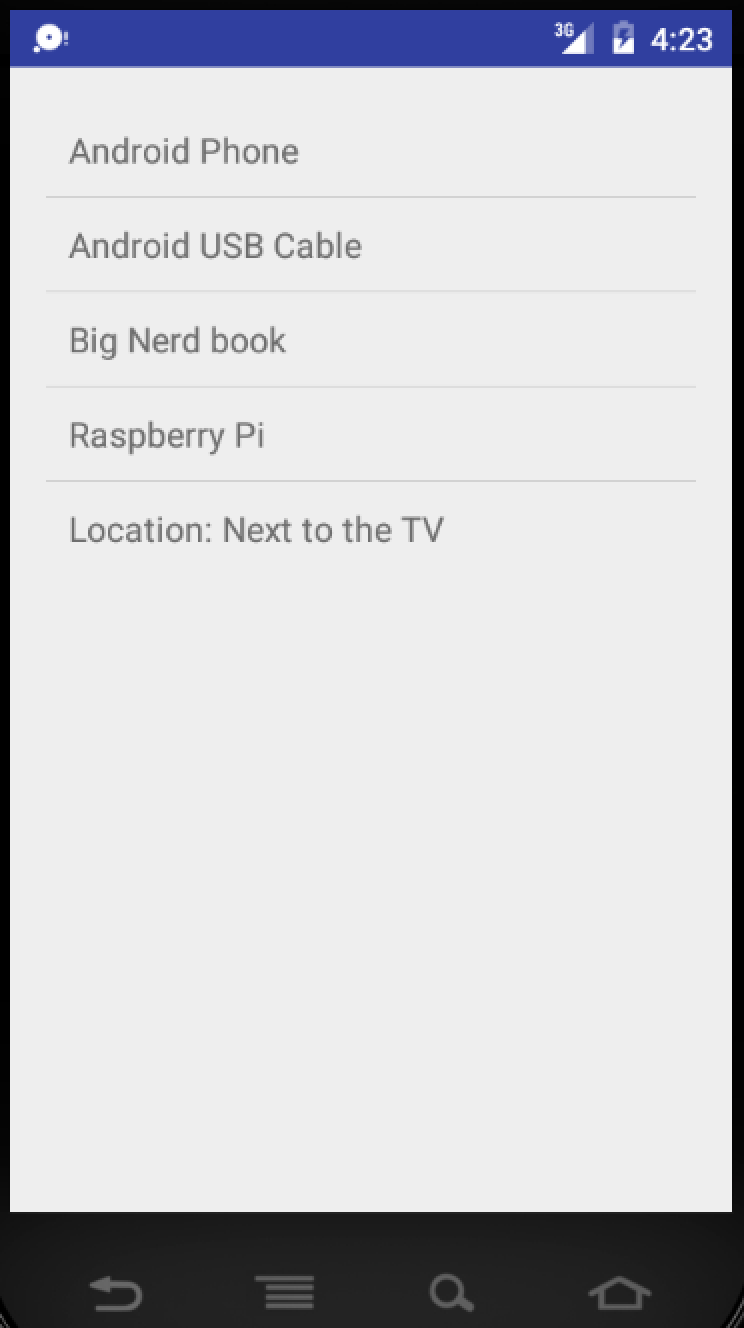
\includegraphics[width=0.9\linewidth]{List-Portrait.png}
		\caption{Portrait view of the List Activity.}
		\label{fig:list-view-portrait}
	\endminipage\hfill
\end{figure}

When running the Tingle App the first view the user sees is shown in Figure \ref{fig:tingle-view-portrait}. In this view the user can add new things and their whereabouts to the database, search for exists things and finally list all things in the database. Clicking the button \texttt{List of All Things} will open up the List Activity shown in Figure \ref{fig:list-view-portrait}. The list view is a scrollable list showing all items in the database. Tapping an item in the list will toggle the \emph{What} (i.e the name of the item) and \emph{Where} (the location of the item). The user can also delete an item by Long pressing on an item. A popup dialog appears as seen in Figure \ref{fig:delete-verification-dialog}.

\begin{figure}[H]
	\centering
	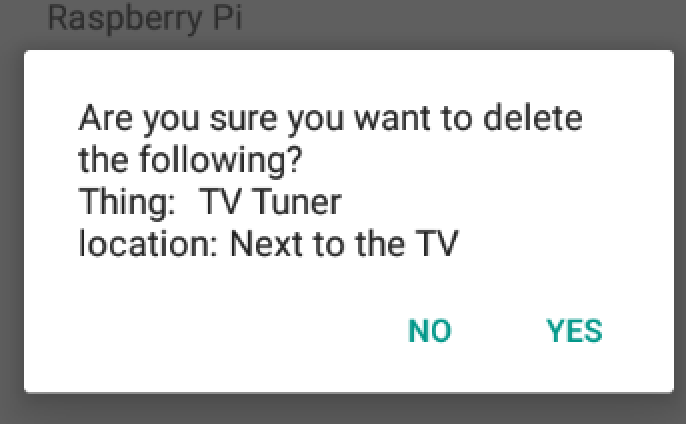
\includegraphics[width=0.3\textwidth]{Longpress-delete-portrait.png}
	\caption{Verification dialog when deleting an item.}
	\label{fig:delete-verification-dialog}
\end{figure}


Changing the orientation to landscape then the two views are show side-by-side. The same functionality applies to this view as they do in portrait mode as described above. The only difference is the removal of the \texttt{List of all things} button since the list is already visible to the right.

\begin{figure}[H]
	\centering
	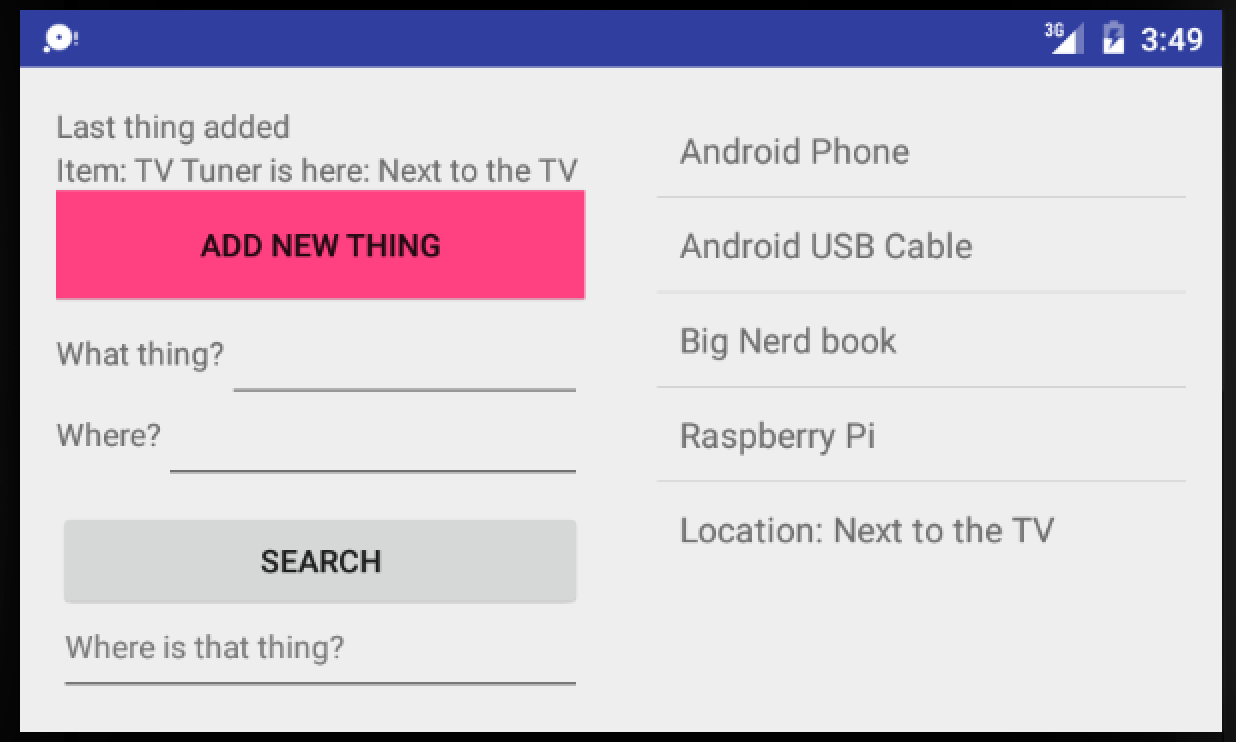
\includegraphics[width=0.6\textwidth]{Landscape-Tap-to-Toggle-Where-and-What.png}
	\caption{Landscape view showing both the main functions as well as the list of things side by side.}
	\label{fig:landscape-main-view}
\end{figure}

\section{Design}
The main design follows the convention explained in chapters 7 and 8 in the book \emph{The Big Nerd Ranch Guide 2nd Edition} using fragments inside Activity classes.
I have separated the main view (\texttt{Tingle}) and the list view (\texttt{List}) into two different activities 
(\texttt{TingleActivity} and \texttt{ListActivity}). This causes some duplication in code since the layout is identical 
but the underlying code depends on which view you currently are in when you turn the device 
from portrait mode to landscape mode. I chose not to make a distinct layout for the list view in 
landscape mode which has resulted in the code being near duplicated between the two Activity classes.
I have tried to separate the fragments so that they do not directly interact with each other in 
order to obtain a more loosely coupled design.
This communication has been moved up to the parent Activity classes instead via interfaces.

\section{Extensions }
A search function has been implemented making it possible for the user to search for an item in 
the database. The user can access this function in the Tingle view.
A delete function has also been implemented making it possible to remove items from the database. To delete an item the user can long-press an item until a verification dialog appears.

\section{Testing}
The testing of the Tingle App has been separated into four different parts using only black-box testing. One for each view and one for each orientation of the device. As can been seen in the tables below the cases are similar for Portrait mode and Landscape mode. This redundant testing is done to make sure there are no unforeseen bugs when changing the orientation.

\begin{figure}[H]
	\renewcommand*{\arraystretch}{1.5} % Redefine padding size
	\begin{tabular}{| c | p{3.5cm} | p{3.5cm} | p{3.5cm} |}
		\hline
		{\textbf{ID} } & {\textbf{Test Case} } & {\textbf{Expected Output}} & {\textbf {Actual Output}} \\\hline\hline
		% -- test 1
		A & Running the App & The Tingle view is shown & The Tingle view is shown  \\ \hline
		% -- test 2
		B &	Clicking the \texttt{List of All Things} button opens up a the List view. & The List view is shown. & The List view is shown. \\ \hline
		C & It is possible to add an item to the database. & An item is successfully added to the database. & An item is successfully added to the database. \\ \hline
		D & It is possible to search for an item in the database. & A Toast is displayed showing the location of the found item. & A Toast is displayed showing the location of the found item. \\ \hline
		E & Clicking \texttt{List of All Things} opens up a the List view. 
     Clicking the android back button navigates back to the Tingle view & User is successfully navigated back to the Tingle view. & User is successfully navigated back to the Tingle view.  \\ \hline
	\end{tabular}
	
	\caption{Test cases of the Tingle view in Portrait mode.}
	\label{tab:test-cases-tingle-portrait}
\end{figure}

\begin{figure}[H]
	\renewcommand*{\arraystretch}{1.5} % Redefine padding size
	\begin{tabular}{| c | p{3.5cm} | p{3.5cm} | p{3.5cm} |}
		\hline
		{\textbf{ID} } & {\textbf{Test Case} } & {\textbf{Expected Output}} & {\textbf {Actual Output}} \\\hline\hline
		% -- test 1
		A & Running the App & Both the Tingle view and List view are shown side-by-side. & Both the Tingle view and List view are shown side-by-side.  \\ \hline
		% -- test 2
		B &	Clicking the \texttt{List of All Things} button in the Tingle view opens up a the List view. & The List view is shown. & The List view is shown. \\ \hline
		C & It is possible to add an item to the database. & An item is successfully added to the database. & An item is successfully added to the database. \\ \hline
		D & It is possible to search for an item in the database. & A Toast is displayed showing the location of the found item. & A Toast is displayed showing the location of the found item. \\ \hline
		E & Changes in Layout compared to Portrait mode & The button \texttt{Lost of All Things} is not present. & The button \texttt{Lost of All Things} is not present. \\ \hline
	\end{tabular}
	
	\caption{Test cases of the Tingle view in Landscape mode.}
	\label{tab:test-cases-tingle-landscape}
\end{figure}

\begin{figure}[H]
	\renewcommand*{\arraystretch}{1.5} % Redefine padding size
	\begin{tabular}{| c | p{3.5cm} | p{3.5cm} | p{3.5cm} |}
		\hline
		{\textbf{ID} } & {\textbf{Test Case} } & {\textbf{Expected Output}} & {\textbf {Actual Output}} \\\hline\hline
		% -- test 1
		A &	It is possible to click an item in the list & Toggles Name / Location of the item.  & Toggles Name / Location of the item. \\ \hline
		B & It is possible to Long click an item in the list. & A dialog is displayed asking if the user wants to delete the clicked item. & A dialog is displayed asking if the user wants to delete the clicked item. \\ \hline
		C & When deleting an item the user can decline the request by pressing \texttt{No}. & The item is not deleted. & The item is not deleted. \\ \hline
		D & When deleting an item the user can accept the request by pressing \texttt{Yes}. & The item is deleted from the list. & The item is deleted from the list. \\ \hline
		E & It is possible to delete all items in the list. & All items are deleted. & All items are deleted. \\ \hline
		F & If there are many items in the database and not all items fit on the screen the user
		can scroll the list. & The list is scrollable. & The list is scrollable. \\ \hline
	\end{tabular}
	
	\caption{Test cases of the List view in Portrait mode.}
	\label{tab:test-cases-list-portrait}
\end{figure}

\begin{figure}[H]
	\renewcommand*{\arraystretch}{1.5} % Redefine padding size
	\begin{tabular}{| c | p{3.5cm} | p{3.5cm} | p{3.5cm} |}
		\hline
		{\textbf{ID} } & {\textbf{Test Case} } & {\textbf{Expected Output}} & {\textbf {Actual Output}} \\\hline\hline
		% -- test 1
		A &	It is possible to click an item in the list & Toggles Name / Location of the item.  & Toggles Name / Location of the item. \\ \hline
		B & It is possible to Long click an item in the list. & A dialog is displayed asking if the user wants to delete the clicked item. & A dialog is displayed asking if the user wants to delete the clicked item. \\ \hline
		C & When deleting an item the user can decline the request by pressing \texttt{No}. & The item is not deleted. & The item is not deleted. \\ \hline
		D & When deleting an item the user can accept the request by pressing \texttt{Yes}. & The item is deleted from the list. & The item is deleted from the list. \\ \hline
		E & It is possible to delete all items in the list. & All items are deleted. & All items are deleted. \\ \hline
		F & If there are many items in the database and not all items fit on the screen the user can scroll the list. & The list is scrollable. & The list is scrollable. \\ \hline
	\end{tabular}
	
	\caption{Test cases of the List view in Landscape mode.}
	\label{tab:test-cases-list-landscape}
\end{figure}

\section{Issues}

As documented in the Test Cases no runtime issues have been found. This is not to say that there are none but the main usage of the application has been proved to work as expected.

The structure of the code on the other hand might not be optimal. There is redundancy with the landscape layout classes for both \texttt{TingleActivity.java} and \texttt{ListActivity.java} as well as the landscape files \texttt{activity\_list.xml} and \texttt{activity\_tingle.xml}. In the current setup these classes and layout files are more or less the same. To rid of this duplication a common dual-mode (landscape mode) layout file could be created.